\documentclass{article}
\usepackage[margin=0.5in]{geometry}
\usepackage{tikz}

\title{4-1 Triangles Lecture Problems}
\date{}
\author{}

\begin{document}
\maketitle

\begin{enumerate}
    \item Find the area of $\triangle ABC$ if $AB = AC = 50$ and $BC = 80$
    \vspace{3cm}
    \item There is a shorter path from $A$ to $B$ in the diagram above.
        What is the shortest distance along the outside of the box from $A$ to $B$?
        \begin{center}
            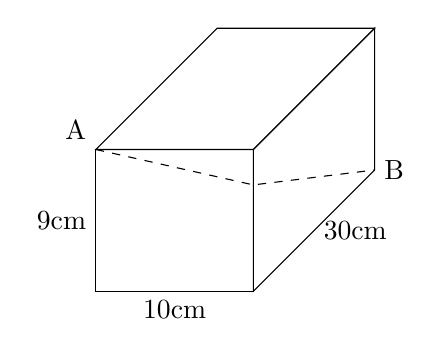
\begin{tikzpicture}
                \coordinate[label=above left:A] (A) at (0,1.8,4);
                \coordinate[label=right:B] (B) at (2,0,0);
                \draw (0,0,4) -- node[left] {9cm} (0,1.8,4) -- (A) -- (2,1.8,4) -- (2,0,4) -- node[below] {10cm} (0,0,4) -- cycle;
                \draw (B) -- node[right] {30cm} (2,0,4) -- (2,0,4) -- (2,1.8,4) -- (2,1.8,0) -- cycle;
                \draw (0,1.8,0) -- (2,1.8,0) -- (2, 1.8, 4) -- (A) -- cycle;
                \draw[dashed] (A) -- (2,1.35,4) -- (B);
            \end{tikzpicture}
        \end{center}
        \vspace{3cm}
    \item What is the height of a STOP sign (regular octagon) whose sides are one foot long?
        \vspace{3cm}
    \item Find the length $AC$ in the regular hexagon $ABCDEF$ if the perimeter of the hexagon is $24$ cm.
        \vspace{3cm}
\end{enumerate}
\end{document}
